\chapter{Methodology}
\label{ch:methodology}

\section{Overview}

This chapter describes the steps that describe the methodology for detecting anomalies of any kind from a large dataset of AIS messages.

The process for detecting anomalies in datasets containing AIS involved several steps that included data engineering techniques such as data cleaning, normalization, transformation, scaling, and finally clustering, as well as a methodology for analyzing the results.

Section \ref{sec:cleaning} describes the methodology used to perform \textbf{data cleaning} of the original data in order to avoid syntactic errors and to perform \textbf{data normalization} of the classical AIS message structure with the aim of lightening the data set and reducing the likelihood of data inconsistencies.

In section \ref{sec:trips} focus shifts to the the anomaly detection object: the \textbf{trip entity}, for which, since it is not explicitly distinguished in each AIS message, a logical-grouping algorithm was required to generate them.

Section \ref{sec:features} contains the \textbf{features engineering} methodology description, that includes the selection and computation of the numerical features for each trip, which are essential for applying the DBSCAN clustering algorithm.

In section \ref{sec:clustering}, the trip data are analyzed with their numerical features and then clustered using the \textbf{DBSCAN algorithm}, obtaining clusters and outliers as result.

In section \ref{sec:importance} the outliers are analyzed in detail, and \textbf{features importance} is carried out thanks to logistic regression technique, which aims to highlight the features with which the outliers were most likely to classify the outliers as such.

At the end, in section \ref{sec:significance} a \textbf{T-test} was ran in order to show the difference in average over each target feature between expected and anomalous AIS Data to measure their statistical meaningful.


\clearpage

\section{Data cleaning and dataset normalization}
\label{sec:cleaning}
    In order to better manage and detect anomalies, a data cleaning task was performed as preliminary steps.
    Indeed, it is likely that an error has occurred in the recording or acquisition of data, resulting in a syntactically anomalous register of information. This has resulted in some isolated records in the dataset that would be better corrected or removed before proceeding with anomaly detection, statistically representing a truly insignificant portion of the source data.
    \\
    Corrupt records in data set fall into the following categories:
    \begin{itemize}
        \item Messages coming from ships without an appropriate identifier.
        \\
        This would have made it difficult to assign the message to a specific ship and thus to a voyage. Messages with the value '0' as \verb|mmsi| (the ship identifier used in this work) and with 'UNAVAILABLE' as \verb|vessel_name| were accordingly removed before we proceeded to the next steps.
        
        \item Messages with coordinates that correspond to land and not to a maritime area.
        This is clearly a data quality error. In order to properly achieve this goal, the python packages cartopy \cite{cartopy} by scitools and shapely \cite{shapely} has been used to detect anomaly coordinates to remove them from the data set.
        
        \begin{minipage}{\linewidth}
        \begin{lstlisting}[language=Python]

import cartopy.io.shapereader as shpreader
import shapely.geometry as sgeom
from shapely.ops import unary_union
from shapely.prepared import prep

# defining the shape of area of earth with a resolution of 10m
land_shp_fname = shpreader.natural_earth(
    resolution='10m', 
    category='physical', 
    name='land')
#join all the land polygons together
land_geom = unary_union(
    list(shpreader.Reader(land_shp_fname).geometries()))
land = prep(land_geom)

# defining function is_land. param msg is the tuple of the message
# return boolean if the messgae was sent from a land point
def is_land(msg):
    return land.contains(
        sgeom.Point(
            msg['longitude'], msg['latitude']))
    
        \end{lstlisting}
        \end{minipage}
        
        
        \begin{figure}[H]
            \centering
            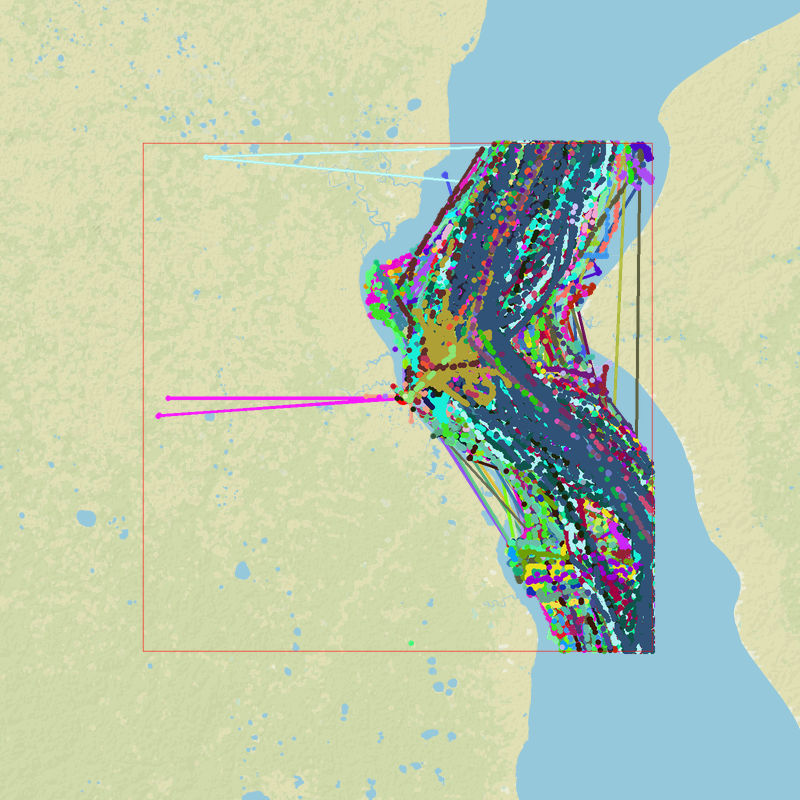
\includegraphics[width=12cm]{Images/2/land-points.png}
            \caption{Presence of wrong vessel coordinates on land}
        \end{figure}
        

        
    \end{itemize}

        
    In addition, some normalization work was done on the data set.
    \\
    At the starting point, all the data about the ship from which the message arrived is contained in the message record. This setting, in addition to weighing down the data set considerably due to a huge amount of redundant data (12 fields out of 33 contain information about the ship and not the message) opens the possibility of inconsistent information.
    \\
    
    \begin{table}[H]
    \begin{tabular}{|c|c|c|c|c|c|}
        \hline
            \textbf{index} & \textbf{imo} & \textbf{vessel\_name} & \textbf{callsign} & \textbf{vessel\_type} & \textbf{vessel\_class} \\
        \hline
            \textbf{5085} & 9120293      & KAPITAN BACHURIKHIN   & UDIZ              & Fishing               & \textcolor{red}{B}      \\
            \textbf{5086} & 9120293      & KAPITAN BACHURIKHIN   & UDIZ              & Fishing               & \textcolor{red}{A}      \\
        \hline
    \end{tabular}
    \caption{Example of data inconsistencies in the data set}
    \end{table}
    \\
    
    Above there is an example of data inconsistency messages 5085 and 5086 comes both from the same vessel but the class registered is different.
    \\
    This is impossible since the class is a vessel-related information.
    
    % PARLARE DELLA NORMALIZZAZIONE
    
    \bigbreak
    
    \begin{table}[H]
    \begin{tabular}{|c|c|c|c|c|c|}
        \hline
            \textbf{index} & \textbf{imo} & \textbf{vessel\_name} & \textbf{callsign} & \textbf{vessel\_type} & \textbf{vessel\_class} \\
        \hline
            \textbf{31699} & 66550      & \textcolor{red}{OTA-883 *!0}   & UDIZ              & Reserved               & A      \\
            \textbf{31699} & 66550      & \textcolor{red}{OTA-883}   & UDIZ              & Reserved               & A      \\
        \hline
    \end{tabular}
    \caption{Example of syntactic errors in the data}
    \end{table}

\clearpage

\clearpage

\section{Trip Generation}
\label{sec:trips}

    As mentioned above, the object of analysis for anomaly detection is the entities \textbf{trips}. These are will be associated with numerical features useful for performing distance-based clustering such as DBSCAN. With the current state of the data, there is no deterministic way to cluster messages by trip (e.g., a trip\_id field in the message dataset).
    \\
    Therefore, it is necessary to define the concept of a trip and write a logical-grouping algorithm that can determine, under certain rules, to which trip each message belongs.
    \\
    The algorithm begins by sorting the receipt of messages chronologically for each ship and performs a scrolling of data to allow grouping along the way.
    When scrolling through the messages in chronological order, the messages were associated to a trip entity. Doing that, the following factors caused it to be interrupted and a new one to be created.
    
    \begin{itemize}
    
    \item A timeframe longer then \verb|SEGMENTS_MAX_DELTA_SECONDS| seconds between two consecutive messages. This variable specifies the minimum time interval between a message A and the next message B, sufficient to consider the two messages as belonging to two different trips. If this is the case, the sequence of successive messages is stopped and message B initiates a new sequence. This variable was given an arbitrary value of \textbf{86400 seconds} (24 hours)
    
    \item The arrival of a message with a change in the status of the ship to "moored". If the ship moors in a port but departs before \verb|SEGMENTS_MAX_DELTA_SECONDS| seconds have elapsed, the script considers two different trips that must be analyzed separately
    \end{itemize}
    \\
    \begin{minipage}{\linewidth}
    \begin{lstlisting}[language=Python]
coords = []
cur_coords = []
last_point = None
rows = load_vessel_file(file_path)
if len(rows) > 1:
    for row in rows:
        timestamp, latitude, longitude, status = row[0], row[1], row[2], row[3]
        # Check if is the first point
        if last_point is None:
             # check if the status is "moored"
            if status == 5:
                continue
            else:
                # register the first point
                cur_coords.append((timestamp, latitude, longitude))
        else:
            # check if the status is "moored"
            if status == 5:

                # get the last point status
                last_point_status = last_point[3]
                if last_point_status == 5:
                    pass
                else:
                    cur_coords.append((timestamp, latitude, longitude))
                    coords.append(cur_coords)
                    cur_coords = []
            else:
                delta_time = (timestamp - last_point[0])
                
                # check if the delta time is more then the max delta time
                if delta_time < settings.SEGMENTS_MAX_DELTA_TIMESTAMP_SECONDS:
                    cur_coords.append((timestamp, latitude, longitude))
                else:
                    if len(cur_coords) > 0:
                        coords.append(cur_coords)
                    cur_coords = [(timestamp, latitude, longitude)]

        last_point = (timestamp, latitude, longitude, status)
    if cur_coords:
        coords.append(cur_coords)
    \end{lstlisting}
    \end{minipage}

\clearpage

\section{Features Engineering}
\label{sec:features}
    One of the most important preliminary steps before applying the DBSCAN clustering method is by far the selection and computation of the \textbf{numerical features} that will become the dimensions we use to describe our entities in space. This phase is called \textbf{Feautures engineering} in the literature. 
     
    The selection of features is so important because the algorithm is able to consider trips as \textit{near} or \textit{far} from each other based on these features. Indeed, a correctly detected anomaly is one that highlights a value of some features that are substantially distant from a group of features with relatively similar values.
    
    Here are the selected trip features and how they were calculated:
    
    %\subsubsection{min\_lat, max\_lat, min\_lon, max\_lon}
    %    These parameters are useful to describe the perimeter in which the ship moved during its voyage. Using %these four features, the DBSCAN clustering algorithm can group voyages with trajectories in very %similar areas.
    
    %\subsubsection{start\_lat, start\_lon, end\_lat, end\_lon}
    %    These parameters are useful to describe the departure and arrival coordinates of the ship during the %voyage. Using these four features, the DBSCAN clustering algorithm can group together voyages with %similar departure and arrival points.
    
    \subsubsection{Relative delay}
    
        The delay accrued by a ship during a voyage could be a good parameter to highlight an anomaly. The latter is calculated by the presence of the parameter eta (Estimated Time of Arrival) parameter in each message. For this purpose, the first message is taken as reference, thus:
        
        \begin{lstlisting}[language=Python]
delay = trip_msgs[0]['eta'] - duration
rel_delay = delay / duration
        \end{lstlisting} 
        
        \verb|delay < 0| $\rightarrow$ the vessel is the ship is ahead of schedule;
        \\
        \verb|delay > 0| $\rightarrow$ the vessel is late.
    
    \subsubsection{Draught Relative Standard Deviation}
    As explained in the Appendix \ref{app:data-description} - AIS Data Description, \textbf{draught} indicates the maximum height of the any part of the vessel under the waterline, in meters. This might be considered a trivial measure, but in the maritime literature it is used as a proxy for the measure of the cargo weight. Therefore, with a statistical measure such as relative standard deviation, we are able to figure out how much this value has deviated during the journey so we may be able to point to an abnormal cargo change.
    
    \begin{lstlisting}[language=Python]
var_coeff_draught = draught_arr.std() / draught_arr.mean() * 100
    \end{lstlisting} 
    
        
    \subsubsection{Average Speed Over Ground}
    
    As explained in the Appendix \ref{app:data-description} - AIS Data Description, \textbf{sog} (Speed Over Ground) indicates the speed of the ship during its voyage. In order to point out anomalies such as excessive deceleration, this feature has been added and calculated as follows:
    
    \begin{lstlisting}[language=Python]
mean_sog = np.array([x['sog'] for x in going_msgs]).mean()
    \end{lstlisting} 
    
    Note that \verb|going_msgs| is different from \verb|trip_msgs|, as the former only considers messages in which the ship is in \textit{Under Way Using Engine} state, making the calculation of these values more meaningful.
            
    \subsubsection{Average Course Over Ground}
    
    The message parameter \textbf{cog}, which indicates the actual direction of motion taking into account compensation for wind and other flow forces, was chosen as trip feature because the average of this value over the entire trip might reveal some anomalies in the trajectory with respect to other similar trips.
    
    \begin{lstlisting}[language=Python]
mean_sog = np.array([x['cog'] for x in going_msgs]).mean()
    \end{lstlisting} 
    
    \subsubsection{Underway using engine time percentage (going\_time)}
    The time the ship spent in the \textit{Under Way Using Engine} state during its voyage can be estimated by summing the delta time frames of each message recorded in that state compared to the immediately preceding message. If a ship has slowed down and spent less time navigating than expected, this feature can highlight that.
    
    \begin{lstlisting}[language=Python]
going_time = 0
for i, msg  in enumerate(trip_msgs):
    # The "Under Way Using Engine" has 5 as status code 
    if msg['nav_status_code'] == 5 and i < len(trip_msgs)-1:
        going_time += trip_msgs[i+1]['timestamp'] - msg['timestamp']
        
going_time_perc = going_time / duration * 100
    \end{lstlisting} 

    \subsubsection{Extra traveled distance}
    Extra distance is the amount in kilometers traveled extra by a ship on a route compared to the route as the crow flies from the point of departure to the point of arrival.
    
        \begin{lstlisting}[language=Python]
extra_distance = actual_distance - ideal_distance
    \end{lstlisting}
    
    Actual distance and ideal distance are computed as follow:
    
    \textbf{Ideal Distance}
    
    The ideal distance feature is closely related to the coordinates of the departure and arrival points. It measures the distance in kilometers as the crow flies from the departure point to the arrival point. This could be useful in figuring out if the ship took some unmotivated detour instead of going straight to the destination.
    \\
    The calculation required the use of geopy \cite{geopy} library.
    
    \begin{minipage}{\linewidth}
    \begin{lstlisting}[language=Python]
ideal_distance =
    geopy.distance.distance(
        (start_lat, start_lon),
        (end_lat, end_lon)
    ).km
    \end{lstlisting} 
    \end{minipage}

    
    \textbf{Actual Distance}
    
    The effective distance, in contrast to the previous one, measures the actual kilometers covered by the ship during its voyage. The calculation of this value is only possible by approximating the actual distance with the sum of the length of the different segments bounded by the arrival of each message.
    
    Also here the geopy \cite{geopy} library was required.
        
    \begin{lstlisting}[language=Python]
actual_distance = 0
for i, g  in enumerate(trip_msgs):
    if i < len(trip_msgs)-1:
        actual_distance += 
            geopy.distance.distance(
                (trip_msgs[i]['lat'], trip_msgs[i]['lon']),
                (trip_msgs[i+1]['lat'], trip_msgs[i+1]['lon'])
            ).km
    \end{lstlisting}
    
    \subsubsection{Duration}

    This feature indicates the duration of the trip. Let \verb|ts_arr| be the array containing the timestamps of each message belonging to the trip. Duration in seconds is calculated as below:
    
    \begin{lstlisting}[language=Python]
duration = max(ts_arr) - min(ts_arr)
    \end{lstlisting}

\clearpage

\clearpage

\section{DBSCAN Clustering}
\label{sec:clustering}

Now that the preliminary steps are complete, we can move on to the core phase of data analysis: \clustering using the DBSCAN algorithm.
\\
Let us first describe the Python libraries that were essential for our work:
\begin{itemize}
\item \textit{numpy} \cite{numpy} which is needed for all operations based on scientific computation;
\item \textit{pandas} \cite{pandas} which is a pillar for data analysis and manipulation;
\item \textit{scikit learn} \cite{sklearn} which provides several easy-to-implement machine learning tools;
\item \textit{matplotlib} \cite{matplotlib} and \textit{seaborn} \cite{seaborn} for data visualization.
\end{itemize}

Let \verb|df| (\textit{DataFrame}) be the container of all previously computed features. A table-like structure where each row is a trip and the columns are represented by the selected features.

\begin{table}[H]
\centering
\begin{tabular}{|r|r|r|r|r|r|r|r|}
\hline
\textbf{duration} & \textbf{sog\_avg} & \textbf{cog\_avg} & \textbf{extra\_dist} & \textbf{rel\_delay} & \textbf{var\_draught} & \textbf{going\_t} \\
\hline
283595 & 1.732044 & 223.012707 & 130.132315 & -0.991326 & 0 & 82.45 \\
5846727 & 0.043140 & 254.626855 & 143.293468 & -0.999579 & 1.2 & 75.23 \\
6688138 & 0.723701 & 105.899139 & 442.814733 & -0.999632 & 7.6 & 99.23 \\
262659 & 5.563536 & 125.331492 & 131.018347 & 41.762289 & 0 & 99.44 \\
177063 & 9.316211 & 201.727804 & 70.746008 & 50.462612 & 14.56 & 100 \\
1094823 & 1.411823 & 97.694134 & 286.579493 & 10.153584 & 0 & 95.55 \\
4939596 & 0.146513 & 192.948035 & 36.856731 & 1.235446 & 8.7 & 15.12 \\
21808 & 3.631579 & 131.307018 & 22.122283 & 146.250275 & 0 & 67.41 \\
94826 & 9.362802 & 59.614976 & 99.741208 & 96.458503 & 0 & 100 \\
90943 & 10.613889 & 44.552778 & 14.546597 & 123.045715 & 4.63 & 93.415656 \\
\hline
\end{tabular}
\caption{Example of trip features dataframe}
\end{table}

\begin{comment}
\subsection{Trip features correlation Analysis}

This phase begins with the calculation of the correlation matrix. Using the Pearson correlation index \verb|[-1,1]|, we can see how much the variables explain each other, or more precisely, how strongly one variable is correlated with another.

A correlation of 1 indicates that two variables are perfectly correlated, while a correlation of -1 indicates that two variables are inversely correlated. Values close to 0 indicate that the two variables are not correlated at all.

\begin{lstlisting}[language=Python]
df.corr()
\end{lstlisting}

In addition a heatmap to interpret the \textbf{correlation matrix} more quickly was used.

\begin{figure}[H]
    \centering
    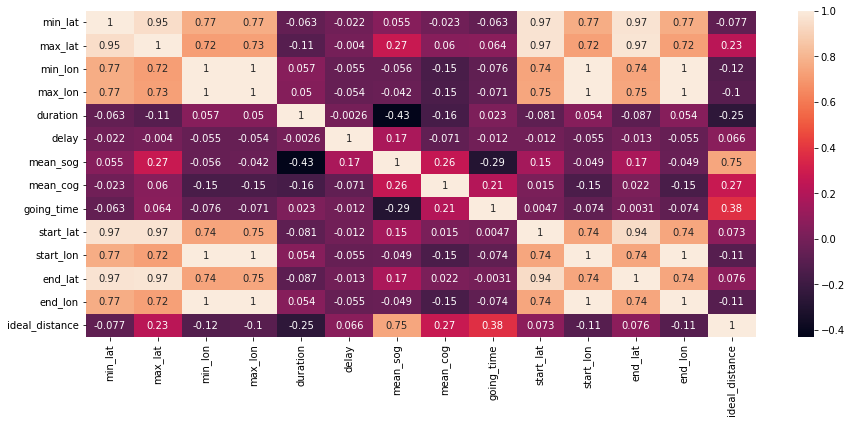
\includegraphics[width=17cm]{Images/2/heatmap.png}
    \caption{Example of trip features correlation heatmap}
\end{figure}

After doing this, we can plot graphs to highlight the correlation between some features.

We can immediately say that the variables \textbf{end\_lat} and \textbf{max\_lat} are strongly correlated (correlation close to 1), as well as for all coordinate pairs.

In contrast \textbf{mean\_sog} and \textbf{duration} are slightly inversely correlated (correlation less than 0).

In contrast, variables such as \textbf{going\_time\_perc} and \textbf{extra\_distance} are weakly correlated (correlation close to 0).

We visualize these pairs of variables through \textbf{scatterplots} to confirm what we observed:

\begin{figure}[H]
    \centering
    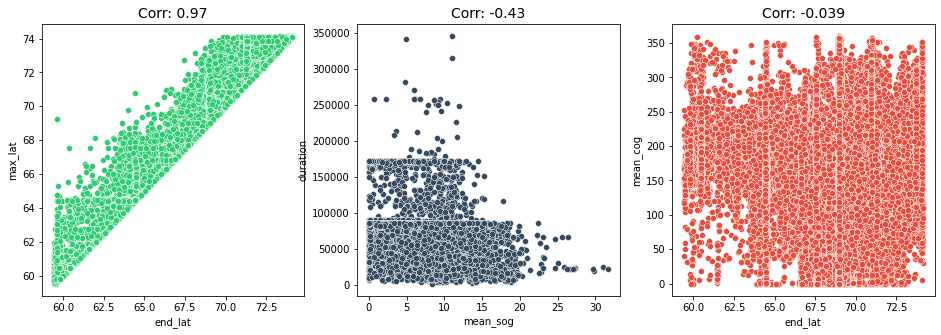
\includegraphics[width=16cm]{Images/2/scatterplots.png}
    \caption{Example of scatterplots with strongly, inversely and weakly correlated features}
\end{figure}
\end{comment}

\subsection{Trip features normalization}

In order to further clean our data before core processing in the clustering phase, this methodology includes removing rows with missing values, i.e., trips that do not contain enough information to compute some features.

After that, a necessary step is the standardization (normalization with null mean and unit standard deviation) of the data set to avoid problems related to the different scaling of variables in practice.

\textbf{Boxplots} are charts that allow us to visualize the distribution of several variables at the same time, in order to verify they are all on the same scale after the normalization.

\begin{lstlisting}[language=Python]
cleaned_df = df.dropna()
scaler = StandardScaler()
scaled_array = scaler.fit_transform(cleaned_df)
scaled_df = pd.DataFrame( scaled_array, columns = cleaned_df.columns )
\end{lstlisting}

\begin{figure}[H]
    \centering
    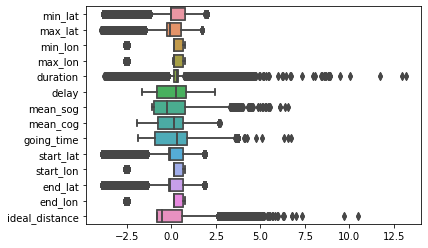
\includegraphics[width=16cm]{Images/2/boxplot.png}
    \caption{Example of boxplot of the trip features after standardization}
\end{figure}


\subsection{DBSCAN implementation}
The DBSCAN is a clustering algorithm that belongs to the category of so-called density-based algorithms, since it only identifies regions of the feature space where the density of points (or observations) is greater.

All observations that are close to each other are grouped into a cluster. Those that appear isolated are referred to as noise.

As mentioned earlier the DBSCAN needs two \textbf{parameters}:

\begin{itemize}
\item $\varepsilon$ which corresponds to the distance within which to search for neighboring points;
\item \textit{n} which corresponds to the minimum number of points in order to compose a cluster.
\end{itemize}

For the sake of brevity we can say that the DBSCAN does nothing more than search for all those clusters whose points are greater than or equal to a number less than $\varepsilon$.

Just as very first step, we give the two parameters an arbitrary value and analyze the results by measuring the number of clusters and the significance of outliers during the hyperparameter phase.

\begin{lstlisting}[language=Python]
dbscan_model = DBSCAN(eps = 0.75, min_samples = 5)
dbscan_model.fit(scaled_df)
\end{lstlisting}

The DBSCAN clustering algorithm has been implemented and within \verb|dbscan_model| we will find all the information regarding the clusters created and the trips considered as \textbf{outliers}. In the testing chapter, we will take a more in-depth look at how to reveal from outliers by applying this methodology to a real data set, together with a graphical representation of the clusters in the section \ref{sec:pca}.

\subsection{Searching for hyperparameters}
\label{sec:tuning}

Since DBSCAN is an unsupervised model it does not enjoy any metrics to calculate its accuracy.

This chapter is only about understanding how to perform the search for hyperparameters, and then explain how the correct parameters were selected in the chapter on testing.
This requires observing how the metrics change as a function of selected hyperparameters. We define the hyperparameters set to be tested:

\begin{minipage}{\linewidth}
\begin{lstlisting}[language=Python]
eps_to_test = [round(eps,1) for eps in np.arange(0.1, 2, 0.1)]
min_samples_to_test = range(5, 50, 5)

print("EPS:", eps_to_test)
print("MIN_SAMPLES:", list(min_samples_to_test))
\end{lstlisting}
\end{minipage}

Let \verb|get_metrics| be a function that receives as input the iterated parameters $\varepsilon$ and \textbf{n}, performs the DBSCAN clustering algorithm, and returns the number of trips considered as outliers and the number of clusters obtained to have all the information in a single data structure and to be able to evaluate the best combination of parameters.

\begin{minipage}{\linewidth}
\begin{lstlisting}[language=Python]
iter = 0
for eps in eps_to_test:
    for min_samples in min_samples_to_test:
        iter += 1
        # Calculating the metrics
        noise_metric, cluster_metric = get_metrics(eps, min_samples, scaled_df, iter)
\end{lstlisting}
\end{minipage}

\section{Feature importance analysis}
\label{sec:importance}

After generating the clusters and outliers, an essential step in analyzing the results obtained is to perform \textbf{feature importance analysis} to understand which features were most likely to have contributed to classify some trips as outliers.

To this end, the \textbf{logistic regression} technique was used, which attempts to model the probability of an event as a linear combination of one or more independent variables. Retrieval of model coefficients is a common method for determining feature importance and creating interpretable machine learning models.


\begin{lstlisting}[language=Python]
# logistic regression

X = data_cluster.drop(columns=['cluster'])
y = data_cluster['cluster'].apply(lambda x: 0 if x == -1 else 1)

X_train, X_test, y_train, y_test = train_test_split(X, y, test_size=0.2, stratify=y, random_state=42)

model = LogisticRegression(max_iter=1000, class_weight='balanced')
model.fit(X_train, y_train) # y = c0 + c1 * x1 + c2 * x2 + ... + c7 * x7
importance = model.coef_[0]
\end{lstlisting}

The section \ref{sec:testing-importance} and appendix \ref{app:testing-results} show the logistic regression results for each cluster obtained with the dataset used as a test.


\clearpage
\section{Results Statistical Significance}
\label{sec:significance}

An indispensable step in assessing the classification quality of a trip as an outlier was to measure the difference between the mean of the outliers' feature value and the same mean value of the cluster under analysis.

In statistics, in fact,the mean of a group of values is a measure that is not stable, i.e., it can be easily influenced. For this reason, a \textbf{T-test} is required to measure the actual difference between the two means.

What is relevant in this context the parameter \textit{p} of the T-test result. If this parameter is smaller than 0.05, it means that the two mean values differ significantly different and consequently the outlier that has become one for this value is sufficiently relevant.

\begin{lstlisting}[language=Python]
ttest = stats.ttest_ind(
    data_cluster[data_cluster['cluster'] == -1][feature],
    data_cluster[data_cluster['cluster'] != -1][feature])
pvalue = ttest.pvalue
\end{lstlisting}


\section{Anomalies evaluation}
Entrambi la logistic regression per la feature importance e il T-test per la statistical significance sono tecniche utilizzate al fine di valutare le anomalie risultanti dal DBSCAN.

Più nel dettaglio il modello trainato della logistic regression per ogni cluster è servito a classificiare le feature in ordine di importanza e ottenendo un'accuratezza del modello.

Per ogni modello e per ogni feature il p value del T-test è stato valutato al fine di considerare solo anomalie con differenze di medie nel valore significativi.

In numeri, sono state considerate solo anomalie collegate a features con:
\begin{itemize}
\item model accuracy > 0.8
\item \textit{p value} < 0.05
\end{itemize}
